In Folgenden sind die während des Versuchs aufgenommenen Daten tabellarisch dargestellt und die 
mit Hilfe des digitalen Oszilloskops aufgenommenen Bilder, zur Veranschaulichung der angezeigten Signale,
eingebunden. An entsprechender Stelle sind Erklärungen zu den Messwerten und Rechnungen gegeben.   

\subsection{Aufbau der Schaltung}
	\cref{fig:AufbauSig1} und \ref{fig:AufbauSig2}, sowie die in den nachfolgendem \cref{sec:ohneNoise} befindlichen Abbildungen zeigen die Veränderung des, vom Oszilloskop angezeigten Signals 
	beim sukzessiven Aufbau der Schaltung und Durchführung des Versuchs.
	Das Signal $U_{sig}$ aus dem \emph{Oscillator Output} ist in seiner Amplitude variabel, wohingegen das Referenzsignal $U_{ref}$ 
	aus dem \emph{Reference Output} mit $\hat{U}_{ref} = \SI{6.6(1)}{\volt} $ eine konstante Amplitude.   
	\cref{fig:AufbauSig1} zeigt das durch den Vorverstärker (mit Gain: 1) verstärkte Signal $U_{sig}$  und \cref{fig:AufbauSig2} 
	zeigt das Referenzsignal $U_{ref}$.
	
	\begin{figure}[!h]
		\centering
		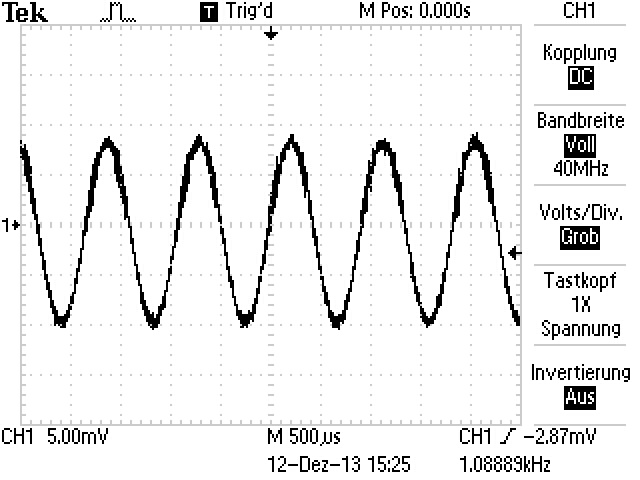
\includegraphics[scale=0.4]{Grafiken/Signalspannung.jpg}
		\caption{Verstärkte Signalspannung $U_{sig}$}
		\label{fig:AufbauSig1}
	\end{figure}
	
	\begin{figure}[!h]
		\centering
		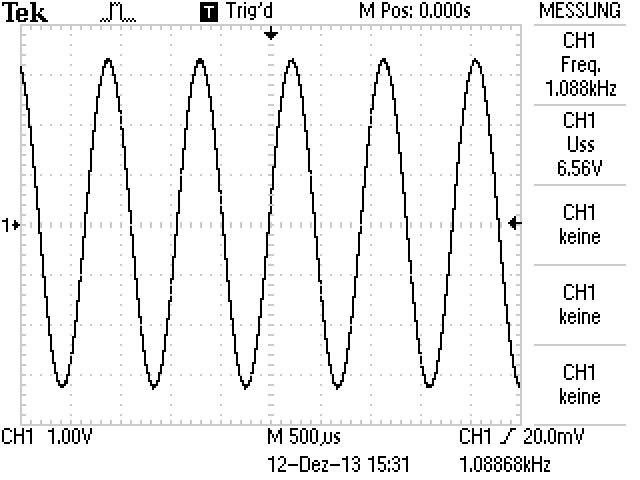
\includegraphics[scale=0.4]{Grafiken/Referenzspannung.jpg}
		\caption{Referenzspannung $U_{ref}$}
		\label{fig:AufbauSig2}
	\end{figure}

	Die durch die Mischung von $U_{sig}$ und $U_{ref}$ veränderten Signalformen sind im folgenden \cref{sec:ohneNoise} dargestellt.
\subsection{Messung ohne Noise-Generator}\label{sec:ohneNoise}
	In den \crefrange{fig:Phase1}{fig:Phase5} sind die am Oszilloskop zu beobachtenden Signale zu sehen, wobei die Phasendifferenz
	bei \cref{fig:Phase1} $\phi = 0$ ist und zur jeweils nächsten Abbildung um $\sfrac{\pi}{6}$ erhöht wird.
	
		\begin{figure}[!h]
			\centering
			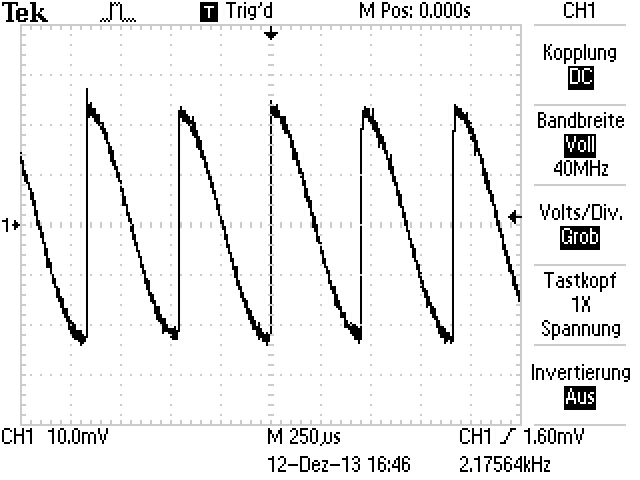
\includegraphics[scale=0.4]{Grafiken/Phase_1.jpg}
			\caption{Mischungssignal mit $\phi = 0$}
			\label{fig:Phase1}
		\end{figure}
		
		\begin{figure}[!h]
			\centering
			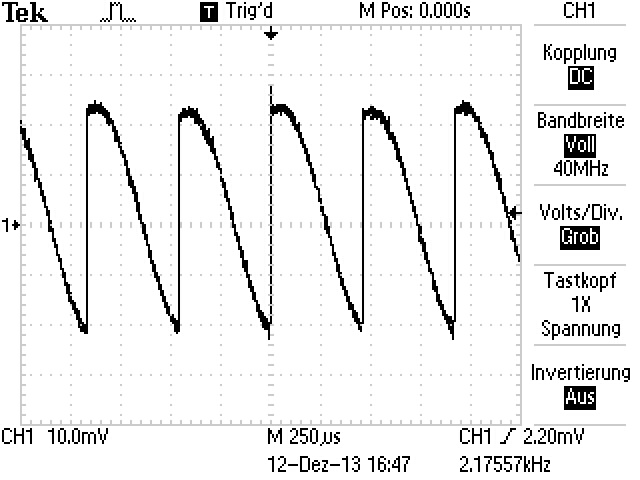
\includegraphics[scale=0.4]{Grafiken/Phase_2.jpg}
			\caption{Mischungssignal mit $\phi = \frac{\pi}{6}$}
			\label{fig:Phase2}
		\end{figure}
		
		\begin{figure}[!h]
			\centering
			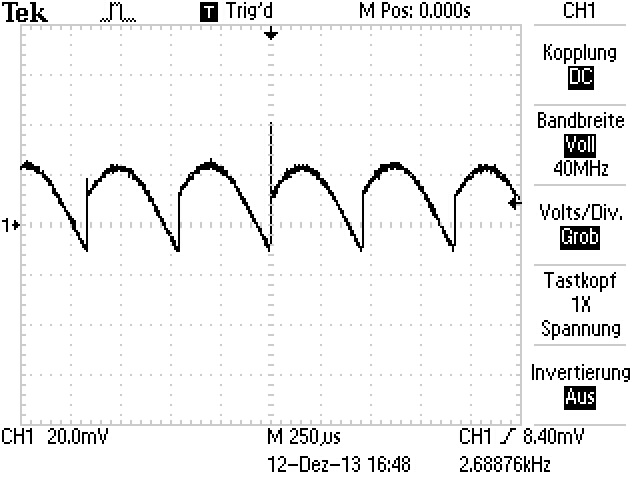
\includegraphics[scale=0.4]{Grafiken/Phase_3.jpg}
			\caption{Mischungssignal mit $\phi = \frac{\pi}{3}$}
			\label{fig:Phase3}
		\end{figure}

		\begin{figure}[!h]
			\centering
			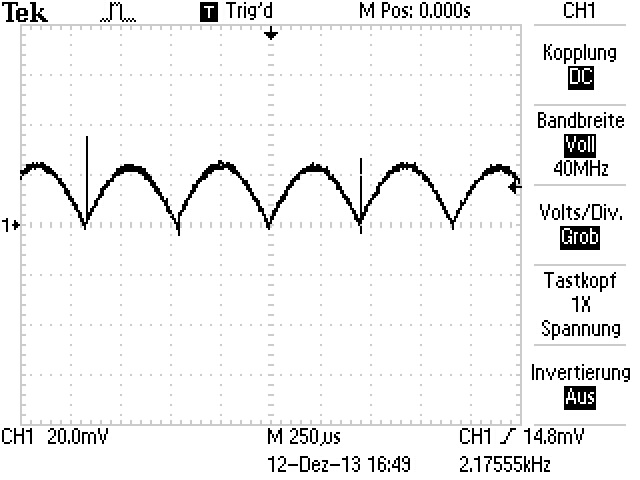
\includegraphics[scale=0.4]{Grafiken/Phase_4.jpg}
			\caption{Mischungssignal mit $\phi = \frac{\pi}{2}$}
			\label{fig:Phase4}
		\end{figure}

		\begin{figure}[!h]
			\centering
			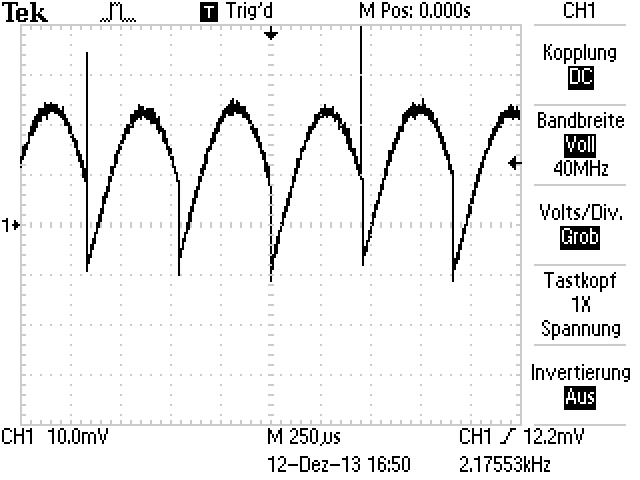
\includegraphics[scale=0.4]{Grafiken/Phase_5.jpg}
			\caption{Mischungssignal mit $\phi = \frac{2\pi}{3}$}
			\label{fig:Phase5}
		\end{figure}

	Durch die Integration des Signals durch den Tiefpass erhält man eine konstante Gleichspannung $U_{out}$,
	deren Form am Beispiel für $\phi = 0$ in \cref{fig:Uout} dargestellt.
	 
	
		\begin{figure}[!h]
			\centering
			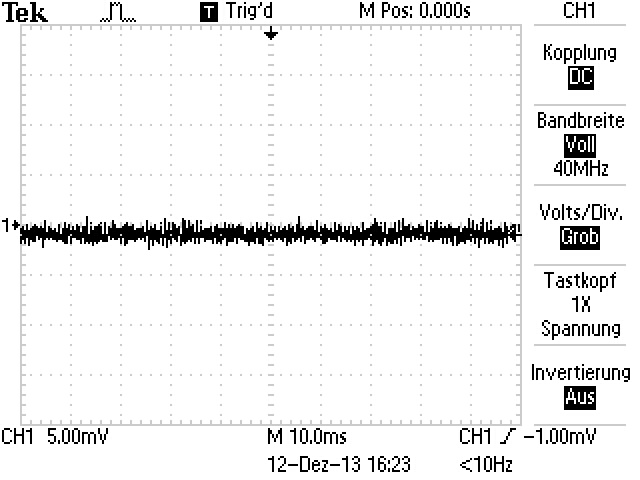
\includegraphics[scale=0.4]{Grafiken/IntegrierteSpannung.jpg}
			\caption{Integriertes Ausgabesignal für $\phi = 0$}
			\label{fig:Uout}
		\end{figure} 
	
	Die Messwerte für diese Ausgabespannung $U_{out}$ sind zusammen mit der entsprechenden Phase in \cref{tab:ohneNoise} eingetragen. 

	\begin{table}[!h]
	\centering
	\begin{tabular}{|c|c|c|}
		\hline
		Phase & Spannung & Spannung\\
		$\phi\,[\si{\degree}]$ & $U_{out}\,[\si{\volt}]$ & $U_{0}\,[\si{\volt}]$\\\hline\hline
		\num{0.000}  & \num{-0.0005(3)}  & - \\
		\num{30.000}  & \num{0.0055(3)}  & \num{0.0173(8)} \\
		\num{60.000}  & \num{0.0130(5)}  & \num{0.0236(9)} \\
		\num{90.000}  & \num{0.0150(5)}  & \num{0.0236(8)} \\
		\num{120.000}  & \num{0.0140(5)}  & \num{0.0254(9)} \\
		\num{150.000}  & \num{0.0070(5)}  & \num{0.022(2)} \\
		\num{180.000}  & \num{0.0010(3)}  & - \\
		\num{210.000}  & \num{-0.0045(3)}  & \num{0.0141(8)} \\
		\num{240.000}  & \num{-0.0120(5)}  & \num{0.0218(9)} \\
		\num{270.000}  & \num{-0.0140(5)}  & \num{0.0220(8)} \\
		\num{300.000}  & \num{-0.0130(5)}  & \num{0.0236(9)} \\
		\hline
	\end{tabular}
	\caption{Messwerte der Messung ohne Noise-Generator \label{tab:ohneNoise}}
\end{table}


	
	An der grafischen Darstellung dieser Messwerte in \cref{fig:ohneNoise} ist festzustellen, das die aufgenommene Messwerte nicht dem
	durch die Theorie prognostiziertem Verlauf von \cref{eq:Uout}, mit der Proportionalität zu $\cos(\phi)$ folgen, sondern Proportional 
	zu $\sin(\phi)$ verlaufen. Daher wird für die weitere Bearbeitung dieser Messwerte anstelle von \cref{eq:Uout} die Gleichung 
	\begin{empheq}{equation}
			U_{out} = \frac{2}{\pi}U_{0}\sin(\phi)
			\label{eq:Uout_sin}
	\end{empheq}     
	verwendet.   
	
		\begin{figure}[!h]
			\centering
			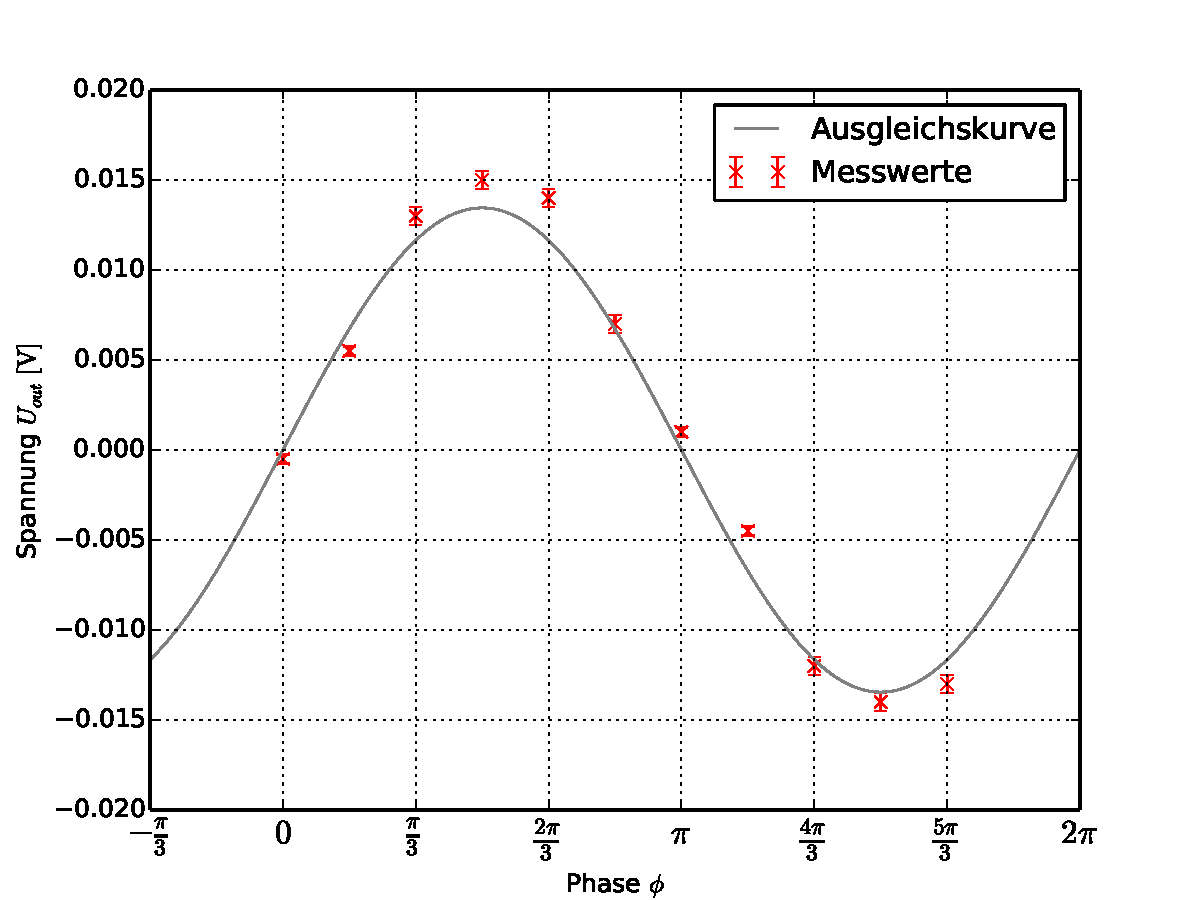
\includegraphics[scale=0.75]{Grafiken/OhneNoise.pdf}
			\caption{Verlauf der Messwerte ohne Rauschen mit Ausgleichskurve}
			\label{fig:ohneNoise}
		\end{figure} 
	
	Die in \cref{fig:ohneNoise} dargestellte Theoriekurve hat dabei die Form $U(\phi) = U_{0} \sin{\phi}$ mit 
	der Amplitude $U_{0} = \SI{0.0135(8)}{\volt}$, welche mit Hilfe der Python-Bibliothek SciPy \cite{SciPy} bestimmt wurde.
	
	Durch Umstellen von \cref{eq:Uout_sin} erhält man die ebenfalls in \cref{tab:ohneNoise} eingetragenen Werte für die 
	Amplitude der Signalspannung $U_{0}$ nach der Gleichung
	\begin{empheq}{equation}
			U_{0} = \frac{\pi}{2}\frac{U_{out}}{\sin(\phi)}.
			\label{eq:U0}
	\end{empheq}  
	Der Mittelwert dieser Werte ergibt sich zu 
	\begin{empheq}{equation}
			\mean{U_{0}} = \SI{0.022(1)}{V},
			\label{eq:U0_mean}
	\end{empheq}  	
	wobei für den angegebene Fehler die Abweichung vom Mittelwert berechnet und keine Fehlerfortpflanzung verwand wurde, da dieser 
	Fehler klein gegen über der angegebenen Abweichung ist.
	 
\subsection{Messung mit Noise-Generator} \label{sec:mitNoise}
	Die Messwerte der Messung mit zwischengeschaltetem Noise-Generator sind in \cref{tab:mitNoise} zusammen mit denen aus diesen
	Werten berechneten Signalspannungsamplituden $U_{0}$ eingetragen.
	
	\begin{table}[!h]
	\centering
	\begin{tabular}{|c|c|c|}
		\hline
		Phase & Spannung & Spannung\\
		$\phi\,[\si{\degree}]$ & $U_{out}\,[\si{\volt}]$ & $U_{0}\,[\si{\volt}]$ \cref{std:U0}\\\hline\hline
		\num{0}  & \num{0.0005(3)}  & - \\
		\num{30}  & \num{-0.0020(3)}  & \num{0.0063(8)} \\
		\num{60}  & \num{-0.0050(3)}  & \num{0.0091(5)} \\
		\num{90}  & \num{-0.0060(3)}  & \num{0.0094(4)} \\
		\num{120}  & \num{-0.0055(3)}  & \num{0.0100(5)} \\
		\num{150}  & \num{-0.0025(3)}  & \num{0.0079(8)} \\
		\num{180}  & \num{0.0000(3)}  & - \\
		\num{210}  & \num{0.0020(3)}  & \num{0.0063(8)} \\
		\num{240}  & \num{0.0060(3)}  & \num{0.0109(5)} \\
		\num{270}  & \num{0.0070(3)}  & \num{0.0110(4)} \\
		\num{300}  & \num{0.0065(3)}  & \num{0.0118(5)} \\
		\hline
	\end{tabular}
	\caption{Messwerte der Messung mit Noise-Generator \label{tab:mitNoise}}
\end{table} 
	
	Als Mittelwert der berechneten Signalspannungsamplituden erhält man
	\begin{empheq}{equation}
			\mean{U_{0}} = \SI{-0.092(6)}{V}
			\label{eq:U0Noise_mean}
	\end{empheq}	
	und auch hier ist der angegeben Fehler die Abweichung vom Mittelwert.
	
	In \cref{fig:mitNoise} sind die Messwerte zusammen mit einer Ausgleichskurve der Form $U(\phi) = U_{0} \sin{\phi}$ mit 
	$U_{0} = \SI{-0.0063(3)}{\volt}$ aufgetragen.

	\begin{figure}[!h]
		\centering
		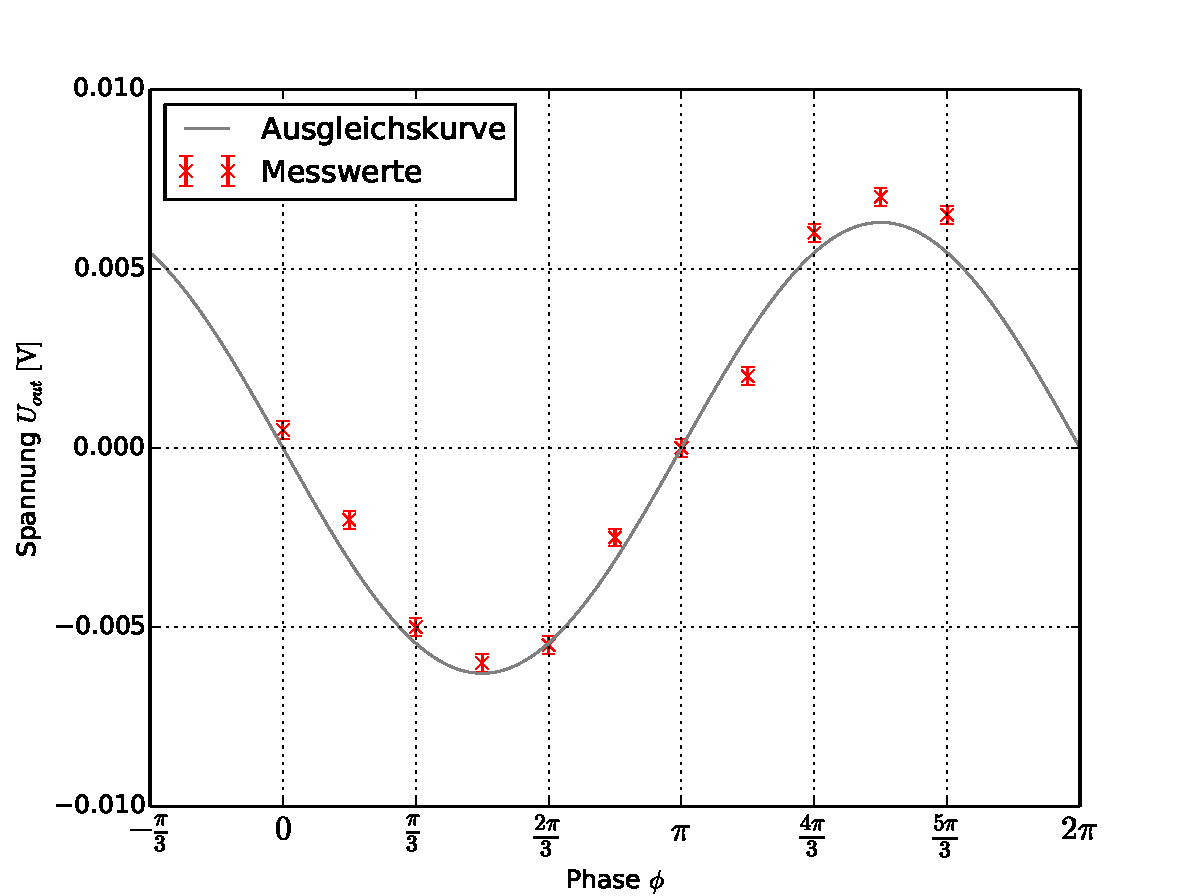
\includegraphics[scale=0.75]{Grafiken/MitNoise.pdf}
		\caption{Verlauf der Messwerte mit Rauschen mit Ausgleichskurve}
		\label{fig:mitNoise}
	\end{figure} 
\subsection{Messung der Intensität einer LED in Abhängigkeit  \\des Abstands} \label{sec:Abstand}
	Die Messwerte für den Abstand und der am Lock-In-Verstärker abgelesenen Spannung als Maß der Lichtintensität
	sind in \cref{tab:Abstand} zu finden. 
	
	\begin{table}[!h]
	\centering
	\begin{tabular}{|c|c|}
		\hline
		Abstand & Spannung\\
		$r\,[\si{\meter}]$ & $U_{out}\,[\si{\volt}]$\\\hline\hline
		\num{0.026(1)}  & \num{0.0180(5)} \\
		\num{0.046(1)}  & \num{0.0100(5)} \\
		\num{0.066(1)}  & \num{0.0060(5)} \\
		\num{0.086(1)}  & \num{0.0040(5)} \\
		\num{0.106(1)}  & \num{0.0025(3)} \\
		\num{0.126(1)}  & \num{0.0020(3)} \\
		\num{0.146(1)}  & \num{0.0015(3)} \\
		\num{0.166(1)}  & \num{0.0010(3)} \\
		\num{0.186(1)}  & \num{0.0008(3)} \\
		\num{0.206(1)}  & \num{0.0005(3)} \\
		\num{0.226(1)}  & \num{0.0003(3)} \\
		\num{0.401(1)}  & \num{0.0000(3)} \\
		\hline
	\end{tabular}
	\caption{Messwerte der Intensität im Abstand $r$ \label{tab:Abstand}}
\end{table}
	
	Dabei wurden während der Messungen zwischen $r = \SI{0.226(1)}{\meter}$ und $r_{max} = \SI{0.401}{\meter}$ 
	noch Veränderungen der Spannung festgestellt, die jedoch kleiner als der Ablesefehler waren und somit nicht bestimmt
	werden konnten. Bei Abständen $r > r_{max}$ konnten keine Spannungsveränderungen mehr festgestellt werden.
	Die Messwerte sind in \cref{fig:Abstand} grafisch dargestellt und durch eine Ausgleichskurve ergänzt, die 
	die Form $U = U_{0}r^{-2}$ mit $U_{0}= \SI{0.13(1)}{\volt}$ hat. Die Antiproportionalität zu $r^{2}$, ist an
	zunehmen, da es sich bei der LED um eine Punktquelle von elektromagnetischer Strahlung handelt, für deren Intensität
	diese Proportionalität gilt. Dies sei hier kurz gezeigt:
	
	Bezeichnetet $S$ die Intensität einer elektromagnetischen Kugelwelle, so ist die Strahlungsleistung $P$ gegeben durch
	\begin{empheq}{equation*}
		P = \int{S}\dif A
	\end{empheq}    
	Betrachtet man des Flächenelement einer Kugeloberfläche $\dif A = r^{2} \sin(\theta) \dif\phi \dif\theta$ ergibt das Integral:
	\begin{empheq}{equation*}
	 	P =  4\pi r^{2} \cdot S
	\end{empheq}  
	woraus folgt
	\begin{empheq}{equation*}
	 	S = \dfrac{P}{4\pi r^{2}} \propto \dfrac{1}{r^{2}}
	\end{empheq} 
	